\chapter{Einführung in Internet of Things}
\section{Übersicht}
Das Internet der Dinge unterscheidet sich in einigen Aspekten vom klassischen Internet. End-Benutzer haben über sogenannte Terminals wie Laptops oder Smartphones über die globale Internet Infrastruktur kommuniziert \cite{MiorandiSicariPellegriniChlamtac12}. Diese Terminals wurden meist von Benutzern eingeschaltet, benutzt und wieder ausgeschaltet. Damit Geräte mit dem Internet auf sinnvolle Art und Weise kommunizieren konnten, war eine manuelle Tätigkeit von Benutzern notwendig \cite{Radovici15}. Beispiele dafür sind das Abrufen von E-Mails, Surfen im Web, Streaming von Videos oder Spielen von Online Games \cite{MiorandiSicariPellegriniChlamtac12}.

Mit \glqq Internet of Things\grqq{} (IoT) wird eine andere Philosophie verfolgt. Es gibt keine einheitliche Definition und Abgrenzung von IoT. Grundsätzlich versucht man Objekte und Gegenstände, welche im klassischen Sinne des Internets nicht berücksichtigt wurden, ans Netz anzuschliessen. Mit minimalen menschlichen Eingriffen sollen diese Geräte Daten sammeln, austauschen und aufgrund von Software und Algorithmen Entscheidungen treffen \cite{RoseEldridgeChapin15}. Man spricht im Zusammenhang von \glqq Things \grqq{} auch von \glqq Smart Devices\grqq{} oder \glqq Smart Objects\grqq .
\subsection{Smart Objects}
Smart Objects oder auch \glqq Things\grqq{} ergänzen das herkömmliche Internet um eine Vielzahl neuartiger Teilnehmer. Man ist versucht, die mit dem Internet erschaffene virtuelle Welt mit Objekten der tatsächlichen \glqq echten\grqq{} Welt zu verbinden. Der Begriff \glqq Smart\grqq{} ist seit der Erscheinung des iPhones weltweit bekannt. Er beschreibt die Fähigkeit eines Objekts mit dem Internet zu kommunizieren. 


Während Smartphones oder Smart-TVs noch als herkömmliche Internet Terminals angesehen werden können, so erweitern die Smart Objects das bisherige Internet um eine neue Art von Teilnehmer. Smart Objects lassen sich wie folgt beschreiben:
\begin{itemize}
\item	haben eine physikalische Repräsentation mit Eigenschaften wie Form und Grösse
\item	haben Mindestmass an Kommunikationsfunktionalitäten wie Request/Reply
\item	besitzen eine UID (unique identifier)
\item	haben mindestens einen Namen und eine Adresse
\item	besitzen ein Mindestmass an Rechenfähigkeiten
\item	besitzen Sensoren, um physikalische Erscheinungen wie Druck, Licht, Temperatur, etc. zu messen
\end{itemize}

Der letzte Punkt in der oberen Definition beschreibt den tatsächlichen Unterschied zu herkömmlichen Devices im Internet. Konzeptionell liegt bei IoT der Fokus mehr auf Daten und Informationen von physikalischen Objekten als bei Punkt-zu-Punkt Kommunikation von Terminals \cite{MiorandiSicariPellegriniChlamtac12}.

\newpage

\section{Einsatzgebiete}
Das ''Internet of Things'' hat viele Einsatzmöglichkeiten und wir stehen erst am Anfang. Es werden immer neue Einsatzbereich entdeckt und vorhandene optimiert und erweitert. Um die Einsatzmöglichkeiten aufzuzeigen, wird hier das Beispiel ''Gesundheitsvorsorge'' genauer gezeigt.
\subsection{Allgemein}
Die Gesundheitsvorsorge ist ein riesiger Bereich, welche alle Menschen betrifft und enorme Kosten verursacht. Heutzutage wird noch sehr viel manuell erledigt. In naher Zukunft wird sich das ändern und das Internet der Dinge wird immer wichtiger, um die bestmögliche Behandlung jedes Patienten sicherzustellen. IoT bringt noch viele weitere Verbesserungen und in Zukunft werden immer neue Einsatzgebiete gefunden. Hier wird nur ein kleiner Teil beschrieben. 
\subsection{Im Alltag}
\subsubsection{Selbstüberwachung}
In den letzten paar Jahre ist die Selbstüberwachung zu einem riesigen Thema geworden. Firmen wie Apple oder Fitbit haben diesen Bereich stark gefördert. So gibt es heute schon für mehrere Körperdatensensoren, die alles Überwachen. Ein Beispiel dafür sind die Smartwatches. Diese können bereits heute den Puls rund um die Uhr überwachen oder sie zählen die Schritte mit. So kann jeder sein eigenes Fitnessprofil von sich erstellen.
Ein weiteres Beispiel findet man bei Patienten, welche Medikamente verabreicht bekommen. Da Medikamente häufig vergessen werden, gibt es kluge Medikamentenspender, welche den Patienten benachrichtigen, wenn dieser die Medikamente nicht genommen hat.
\subsubsection{Fernüberwachung}
Neben der Selbstüberwachung gibt es auch noch die Fernüberwachung. Dabei wird der Patient vom Pflegepersonal überwacht und bei kritischen Situationen kann sofort gehandelt werden. Für Rollstuhlfahrer oder Senioren gibt es zum Beispiel ein Falldetektor. Falls der Patient umfällt, reagiert der Sensor und meldet diesen Unfall direkt an das Pflegepersonal. So kann schnell reagiert und dem Patienten geholfen werden. Auch das Überwachen der Patientenwerte kann so über das Internet sichergestellt werden. Durch eine kontinuierlich Abfrage der Werte, ist die Reaktionszeit enorm kleiner, als beim manuellen messen. Hierfür benötigt man Pflegepersonal vor Ort.
\subsection{Im Spital}
\subsubsection{Patientenzimmer}
Durch die komplette Überwachung des Patienten in seinem Zimmer, verkürzt sich die Reaktionszeit enorm. Der Patient wird zwar schon überwacht, aber durch die Anbindung an das Internet wären weitere Verbesserungen möglich. So kann man bei gewissen Problemen nicht nur das Pflegepersonal alarmieren, sondern zum Beispiel auch direkt benötigtes Personal aus anderen Spitälern anordnen. Auch könnte man die Messdaten aus der Fernüberwachung mit der aus dem Patientenzimmer verknüpfen und so ein besseres Patientenbild erstellen. Der Patient wäre so lückenlos überwacht und bei Problemen wären die Daten sehr hilfreich.
\subsubsection{Infrastruktur}
In Spitälern werden viele verschiedenen Geräte eingesetzt, welche momentan noch nicht miteinander kommunizieren. Durch die Verknüpfung der Geräte könnte man die Daten verschiedener Geräte miteinander kombinieren und vergleichen, um ein besseres Bild erstellen zu können. Oder auch die Wartung würde viel einfacher werden. Aus der Ferne werden alle Geräte inventarisiert, gewartet und überwacht. So wird bei einem Fehler sofort der Techniker gerufen, damit ein defektes Gerät sofort wieder Einsatzbereit gemacht wird.
 
\newpage

\section{Sensortypen}
Beim Thema ''Internet of Things'' spielen die Sensoren eine zentrale Rolle. Es gibt viele verschiedene Typen von Sensoren, welche unterschiedlichste Daten liefern und man muss daher wissen, wie man mit dem jeweiligen Sensortyp umgeht. 
\begin{figure}[H]
\centering
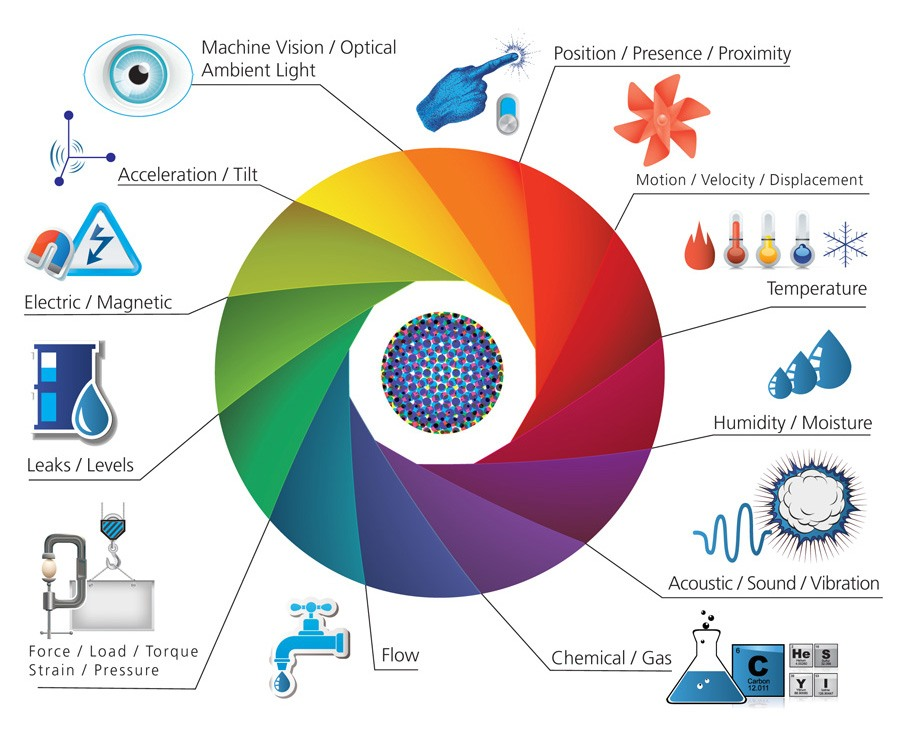
\includegraphics[scale=0.35]{images/sensors.jpg}
\caption{Sensortypen\cite{SensorImage}}
\end{figure}

\subsection{Temperature}%DONE
Temperatursensoren werden in vielen Gebieten eingesetzt. Häufig wird dieser Sensortyp zur Überwachung von Gebäuden eingesetzt, oder hilft bei maschinell hergestellten Esswaren, die richtige Temperatur zu halten. Auch kann ein Bauer diese Sensoren verwenden, um die Bodentemperatur zu Überwachen. So kann man effizienter und gewinnbringender Arbeiten, ohne selber Messungen durchzuführen.
\subsubsection{Bespielgeräte}
\begin{itemize}
\item	Smarte Heizungsteuerungen in einem Haushalt
\item	Wetterstationen
\end{itemize}


\subsection{Acceleration/Tilt}%DONE
Beschleunigungs- und Lagesensoren hat wohl jeder in seiner Hosentasche. Nahezu alle neuen Smartphones haben solche eingebaut. Auch in der Autoindustrie findet man solche sehr häufig. Durch solche Sensoren kann man viele Verschiedene Daten erhalten. So kann man zum Beispiel Bewegungsprofile einer Person erstellen und den Fitnesslevel bestimmen.
\subsubsection{Bespielgeräte}
\begin{itemize}
\item	Schrittzähler (z.B in Smart Watches)
\end{itemize}


\subsection{Acoustic/Sound/Vibration}%DONE
Nicht nur in der Musikbranche sind Akustik- und Soundsensoren sehr wichtig. So wird auch der Lärm in einem Gebiet oder in einer Stadt gemessen, um Verbesserungen der Lebensqualität zu erreichen. Sehr wichtig sind auch die Vibrationssensoren, welche wichtige Daten zu Unterwassererdbeben senden. So können Tsunamis immer früher erkannt werden und retten Leben.
\subsubsection{Bespielgeräte}
\begin{itemize}
\item	Erdbebenwarnsysteme
\item	Sprachsteuerungen
\end{itemize}


\subsection{Chemical/Gas}%DONE
Chemikaliensensoren werden häufig in den Städten mit viel Verkehrsaufkommen eingesetzt. Dadurch wird die Luftqualität bestimmt. Auch in Laboren ist dies ein wichtiger Sensor, um die Qualität oder Reinheit von Gasen zu messen.
\subsubsection{Bespielgeräte}
\begin{itemize}
\item	Smart City Luftüberwachung
\item	Überwachung von gasbetriebenen Geräten
\end{itemize}


\subsection{Electric/Magnetic}
Magnetische Sensoren könnten in verschiedenen Geräten verbaut werden. Zum Beispiel smarte Türschlösser könnten via solchen Sensoren geschlossen oder geöffnet werden. Auch Elektrizitätswerke können diverser solche Sensoren verwenden, um die Systeme zu überwachen.
\subsubsection{Bespielgeräte}
\begin{itemize}
\item	Smarte Schlösser
\item	Stromüberwachung
\end{itemize}


\subsection{Flow}%DONE
Für die Überwachung von Flüssen oder Wasserleitungen werden Flusssensoren verwendet. So können zum Beispiel Wasserversorger den Verbrauch jedes Haushalts über das Internet messen lassen und müssen nicht vor Ort die Zähler ablesen. Oder auch für die Überwachung von Flüssen kann dieser Sensor verwendet werden. So wird man bei zu schnellen und zu vielem Wasser vor Überschwemmungen gewarnt.
\subsubsection{Bespielgeräte}
\begin{itemize}
\item	Smarte Wasserversorgungen
\item	Überschwemmungsschutz
\end{itemize}


\subsection{Force/Load/Torque/Strain/Pressure}%DONE
Im Fitnessbereich gibt es schon seit Jahren mehrere Körperwaagen, welche solche Sensoren verwenden. Man wird gewogen und gleichzeitig sendet das Gerät allerlei Daten an den Cloud-Dienst. Auch Parksysteme oder automatische Wiegesysteme in Lagern sind Beispiele, welche bereits im Einsatz sind. Diese Sensoren sind vielfältig einsetzbar.
\subsubsection{Bespielgeräte}
\begin{itemize}
\item	Wiegesysteme/Körperwaage
\item	Parksysteme
\end{itemize}


\subsection{Humidity/Moisture}%DONE
Ein wichtiger Bestandteil der Luftqualität ist auch die Luftfeuchtigkeit. Diese wird mit diesem Typ gemessen. So können Smart Buildings die Luftfeuchtigkeit laufend messen und immer wieder optimieren. Auch in der Landwirtschaft kann so eine Automation eingeführt werden, damit die Erde immer optimal bewässert ist.
\subsubsection{Bespielgeräte}
\begin{itemize}
\item	Bewässerungsanlagen
\item	Pflanzensensoren
\end{itemize}


\subsection{Leaks/Levels}%DONE
Lecks- und Levelsensoren sind zum Beispiel in der Landwirtschaft notwendig. Die Landwirtschaft benötigt viel Wasser und man möchte unnötige Lecks vermeiden. Ein weiterer wichtiger Einsatzbereich ist die Überwachung von Flüssigkeitsständen, zum Beispiel bei Staudämmen oder in Lagersystemen.
\subsubsection{Bespielgeräte}
\begin{itemize}
\item	Leitungsüberwachungen
\item	Lagerverwaltungen
\end{itemize}


\subsection{Machine Vision / Optical Ambient Light}%DONE
Machine Vision ist ein immer wichtig werdender Sensor. Durch diese kann man den Dingen das Sehen ''lehren''. So sind automatische Eintrittkontrollen möglich. Auch in den SmartCars kommen diese Sensoren zum Einsatz. Da werden durch die Sensoren die Fussgänger, die Fahrbahn oder auch andere Autos erkannt. Bei Optical Ambient Light geht es um Sensoren, welche die Umgebungsbeleuchtung messen und diese Optimal anpassen. So gibt es schon mehrere smarte Leuchtmittel, welche so über das Internet eingestellt werden können.
\subsubsection{Bespielgeräte}
\begin{itemize}
\item	SmartCars
\item	Eintrittskontrollen
\end{itemize}


\subsection{Motion/Velocity/Displacement}%DONE
Bewegungsensoren sind praktische Helfer bei Sicherheitssystemen. Eine zentrale Überwachung von mehreren Gebäuden ist so problemlos möglich. Bei der Pflege von Rollstuhlfahrer wäre zum Beispiel auch eine Falldetektion möglich. Das zentrale Pflegezentrum hätte so eine schnelle Meldung über Unfälle und könnte mehrere Personen überwachen und betreuen.
\subsubsection{Bespielgeräte}
\begin{itemize}
\item	Sicherheitsanlagen
\item	Verkehrsüberwachung
\end{itemize}


\subsection{Position/Presence/Proximity}%DONE
Immer wichtiger wird auch dieser Typ von Sensoren. Durch die Bestimmung von Distanzen oder der Position in einem Raum, ergeben sich viele Einsatzmöglichkeiten. Ein bekanntes Beispiel ist der Abstandssensor bei Autos, um Parkschäden oder Auffahrunfälle zu vermeiden. Oder auch die Gebäudeüberwachung profitiert durch solche Sensoren, da man mehrere Gebäude zentral Überwachen kann.
\subsubsection{Bespielgeräte}
\begin{itemize}
\item	Smarte Parkhäuse
\item	SmartCars
\end{itemize}

\newpage

\section{Architektur}
Man könnte ein IoT System in vier wichtige Gruppen unterteilen: \cite{IoTNetworks}
\begin{itemize}
\item Dinge (things)
\item das lokale Netzwerk
\item das Internet
\item Back-End Services (z.B. Cloud Services)
\end{itemize}
\begin{figure}[H]
\centering
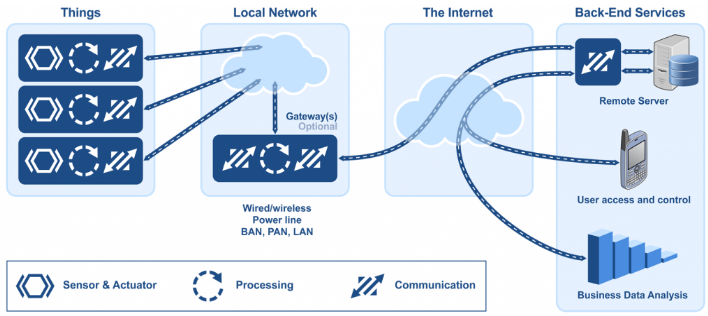
\includegraphics[scale=0.8]{images/iot_system_overview_by_micrium.png}
\caption{IoT Systemübersicht\cite{IoTOverview}}
\end{figure}
Grundsätzlich scheint die Architektur vertraut. Smart Objects kommunizieren über ein lokales Netzwerk mit Diensten im Internet.

Bisher konnten Geräte wie Laptops, PCs und Smartphones beinahe einheitlich mit dem Internet verbunden werden; entweder verkabelt über Ethernet oder drahtlos über ein lokales WLAN oder mobile Netze wie UMTS und LTE. Die Endgeräte verfügten jeweils über viel Rechenleistung, Speicher und ein leistungsfähiges Betriebssystem mit einem vollständig implementierten TCP/IP Stack. 

In einem IoT System muss man von einer grossen Anzahl an Geräten mit Sensoren ausgehen. Diese Geräte verfügen meist über eine extrem niedrige Bandbreite, wenig Speicher und Rechenleistung \cite{CiscoIoTArchitecture}.

Die Kommunikation erfolgt oft nicht vertikal der Architektur, sondern auch horizontal auf derselben Ebene. Sensordevices können beispielsweise miteinander kommunizieren oder Cloud Services Daten der Sensoren untereinander austauschen.
\subsection{Wireless Sensor Netzwerke}
Bei einer Vielzahl von verbundenen Sensoren, welche über einen grossen Bereich verstreut sind, bietet sich ein Wireless Sensor Network (WSN) an. In einem WSN werden die Sensoren nicht direkt mit dem Internet verbunden. Die Daten werden drahtlos von Teilnehmer zu Teilnehmer versendet. Muss ein Datenpaket in ein entferntes Netzwerk wie das Internet, so wird ein Gateway oder Edge Node benötigt.
\begin{figure}[H]
\centering
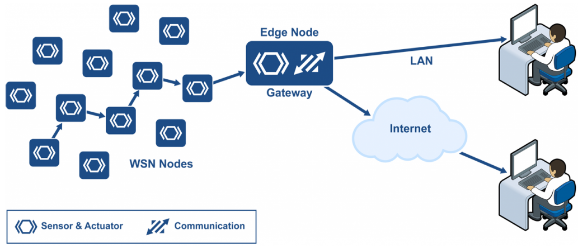
\includegraphics[scale=0.8]{images/iot_wsn_lan_overview_by_micrium.png}
\caption{IoT WSN\cite{IoTWSN}}
\end{figure}
WSN Nodes sind typischerweise günstig im Einkauf. Sie können mit sehr wenig Leistung betrieben werden, dies ermöglicht den Batteriebetrieb. Durch diese Eigenschaften können WSN Nodes einfach, schnell und in sehr grosser Anzahl bereitgestellt werden. 

\section{Kommunikationsmodelle}
Internet of Things verbindet Objekte aus der realen Welt miteinander. Um Objekte aus der Realität in die virtuelle Welt zu transformieren, werden Sensoren verwendet. Es gilt nun, diese Sensoren mit dem Internet zu verbinden.

Um unterschiedliche Bedürfnisse abzudecken, sind verschiedene Arten der Kommunikation entstanden. Die mit Sensoren ausgestatteten Geräte können sich in ihrer Weise, mit dem Internet zu kommunizieren stark unterscheiden.

\subsection{Device-to-Device}
Beim Device-to-Device Kommunikationsmodell kommunizieren mehrere Teilnehmer direkt miteinander (Peer-to-Peer). In diesem Szenario kommunizieren unterschiedliche Glühbirnen drahtlos mit einem Lichtschalter. Denkbar wären sämtliche Anwendungsgebiete aus dem \glqq Smart Home\grqq Bereich. Kommunikation mit dem Internet ist nicht zwingend notwendig. Eine grosse Herausforderung besteht darin, dass mehrere Teilnehmer unterschiedlicher Hersteller miteinander interagieren können. Dazu müssen die Teilnehmer denselben Protokoll-Stack implementieren. 
\begin{figure}[H]
\centering
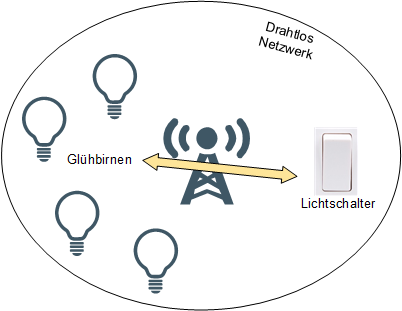
\includegraphics[scale=0.8]{images/device-to-device.png}
\caption{Device-to-Device Kommunikation}
\end{figure}
\subsection{Device-to-Cloud}
Die Gerätehersteller bieten für ihre End-User Cloud-Dienste im Internet an. Die Sensorgeräte kommunizieren direkt End-to-End über TCP/IP mit dem jeweiligen Cloud-Dienst. Die Benutzer können über eine Mobile App oder eine Webseite auf die jeweiligen Sensordaten zugreifen. Häufig wird aufgrund proprietärer Kommunikationsprotokolle ein Vendor-lock-in betrieben. Dies erschwert die Interoperabilität von Sensoren unterschiedlicher Hersteller \cite{RoseEldridgeChapin15}.
\begin{figure}[H]
\centering
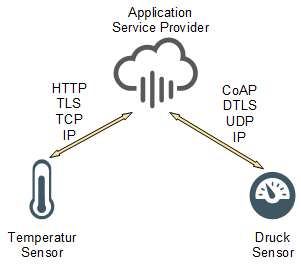
\includegraphics[scale=0.8]{images/device-to-cloud.png}
\caption{Device-to-Cloud Kommunikation}
\end{figure}
\subsection{Device-to-Gateway}
Anstatt einer Ende-zu-Ende Kommunikation zwischen Sensoren und Servern wird in diesem Modell ein Gateway zwischen diesen Komponenten eingesetzt. Sensoren kommunizieren somit nicht direkt mit einem Server. Auf diese Art und Weise können eine grosse Anzahl Sensoren mit Internetdiensten verbunden werden ohne dass die Sensoren selbst über einen direkten Internetzugriff verfügen. Der Gateway muss somit über eine Schnittstelle verfügen, damit Dienste im Internet indirekt mit den Sensoren kommunizieren können. Aus Sicht des Diensts ist es irrelevant, wie der Gateway mit den Sensoren kommuniziert.
\begin{figure}[H]
\centering
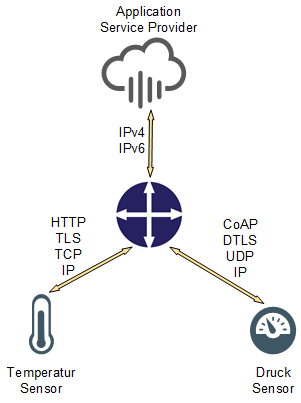
\includegraphics[scale=0.8]{images/device-to-gateway.png}
\caption{Device-to-Gateway Kommunikation}
\end{figure}
\subsection{Back-End Data-Sharing}
Sobald sich die Sensordaten auf einem Server befinden, können diese auf bekannte Weise anderen zur Verfügung gestellt werden. Beispielsweise könnte man den Zustand eines Sensors als JSON Objekt über eine REST-Schnittstelle abfragen. Ein weiterer Serviceprovider muss somit nicht mehr direkt mit den Sensoren kommunizieren. Da Sensordevices oft über limitierte Möglichkeiten verfügen, grössere Datenmengen bereitzustellen, verringert man mit dieser Art der Kommunikation die Anzahl Abfragen auf den Sensordevices. 
\begin{figure}[H]
\centering
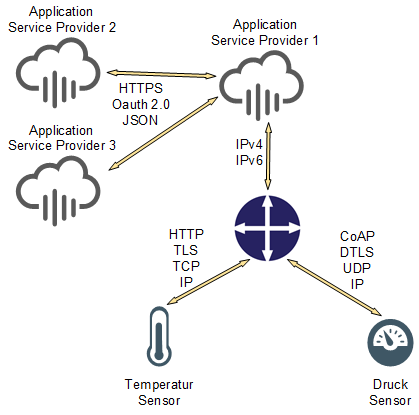
\includegraphics[scale=0.8]{images/backend-data-sharing.png}
\caption{Backend-Data-Sharing Kommunikation}
\end{figure}

\newpage

\section{IoT Kommunikationsprotokolle}
Seit der Entstehung des Internets werden für unterschiedliche Aufgaben Kommunikationsprotokolle entwickelt. Eine grosse Herausforderung war stets die Interoperabilität zwischen Geräten unterschiedlicher Hersteller. Standardisierungsgremien wie die International Standards Organization (ISO) und die Internet Engineering Task Force (IETF) haben in den vergangenen Jahrzehnten Richtlinien und Standardisierung von Kommunikationsprotokollen veröffentlicht. 

Mit zunehmender Popularität des Internets der Dinge sind eine unüberschaubare Menge an proprietären und offenen Kommunikationsprotokollen entstanden. In der Geschichte des Internets hat sich gezeigt, dass sich langfristig nur offene Protokolle durchsetzen werden \cite{Obermaier14}, proprietäre Protokolle hingegen werden aufgrund der fehlenden Interoperabilität niemals eine breite Verwendung finden.
\subsection{Anforderungen}
Bereits heute zeichnen sich die populärsten IoT Kommunikationsprotokolle ab. Um zu verstehen weshalb-, und vor allem in welchen Szenarien welches Protokoll eingesetzt wird respektive werden sollte, muss man sich mit den unterschiedlichen Anforderungen vertraut machen.

Die typischen bekannten Fragen nach der Verbreitung/Unterstützung und Skalierbarkeit stellen sich auch hier. Ebenfalls muss auf die mutmassliche Datenmenge geachtet werden. So dürfte eine vergleichsweise hohe Datenmenge für Geräte, welche über einen direkten, verkabelten Internetzugang verfügen, kein Problem darstellen, während Geräte in einem Mesh-betriebenen WSN wohl über deutlich weniger Bandbreite verfügen dürften.

Weitere Anforderungen wären Realtime Kommunikation, Stromverbrauch, Sicherheit und Network Address Translation (NAT) \cite{Obermaier15}.
\subsection{Request/Response}
Request/Response ist das wohl bekannteste Pattern. Ein Client fordert mittels eines Requests eine Response von einem Service an. Der Service hört auf einkommende Requests, verarbeitet diese und antwortet (Response) den aufrufenden Clients. Request/Response Kommunikation skaliert schlecht, deshalb sollte beim Versenden einer Meldung an viele Teilnehmer auf ein anderes Pattern zurückgegriffen werden. 
\begin{figure}[H]
\centering
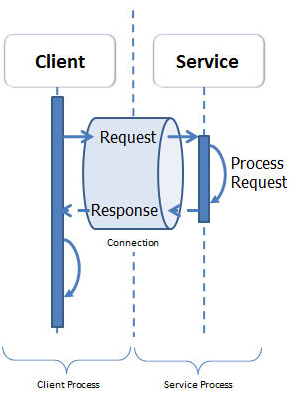
\includegraphics[scale=0.8]{images/request-response.png}
\caption{Request/Response Kommunikation \cite{ReqRes}}
\end{figure}
\subsubsection{HTTP}
In den 1990er Jahren wurde HTTP verwendet um statische HTML-Dokumente übers Internet abzurufen. Bis heute hat sich die grundsätzliche Funktion von HTTP nicht verändert. HTTP bietet über seine Methoden ein umfangreiches Interface für die Request/Response Kommunikation zwischen Clients und Servern über das Internet. 

Aufgrund seiner hohen Verbreitung, Standardisierung und Unterstützung ist HTTP auch im IoT Umfeld beliebt. Für fast jede Programmiersprache und Laufzeitumgebung existieren Libraries, was das Entwickeln sehr angenehm macht. HTTP eignet sich jedoch nicht für alle Anwendungsfälle im IoT Bereich. Für jeden Request wird der gesamte HTTP (und darunterliegende) Header benötigt. Zusätzlich ist das Protokoll textbasiert, was mit dem zusätzlichen, grossen Overhead eine erhebliche Datenmenge bedeuten könnte. Für Endgeräte an Mobilen Netzwerken könnte dies ungeeignet sein \cite{Obermaier15}.

In der Version 1, respektive 1.1 gibt es mit HTTP keine Möglichkeit, echte Push-Meldungen zu versenden. Bei Push-Meldungen sendet der Server eine Response (besser: Nachricht) an den Client ohne vorgängigen Request. In der Version 2 von HTTP sind echte Push-Meldungen vorgesehen, jedoch gibt es wenige Implementation und Erfahrungswerte damit.
\subsubsection{CoAP}
Das Constrained Application Protocol (CoAP) implementiert wie HTTP das Request/Response Pattern \cite{Obermaier15}. Mit CoAP existiert ein massgeschneidertes IoT-Protokoll, welches nach dem REST Paradigma konzipiert wurde. HTTP ist schwergewichtig, hat einen grossen Overhead und generiert damit hohe Datenmengen. Ausserdem ist vor jeder Session den für TCP benötigten 3-Way Handshake nötig. 
 
CoAP wurde entwickelt, um diesen Schwächen von HTTP entgegenzuwirken. Bei sogenannten Low-Power and Lossy Networks (LLN's) sind die Nodes im Vergleich zu herkömmlichen Computersystemen sehr eingeschränkt, was die Verwendung von HTTP schwierig gestaltet. CoAP bietet grundsätzlich folgende Features:\cite{RFC7252}
\begin{itemize}
\item Request/Response Kommunikation zwischen Endpoints	
\item Discovery von Services und Ressourcen
\item URI's und Media Types
\item Kompatibilität mit HTTP
\item Multicast Support
\item sehr kleiner Overhead (Header von 4 Byte)
\item implementiert das Observer Design Pattern
\item UDP als Transportprotokoll
\item Asynchroner Nachrichtenaustausch
\end{itemize}
 
CoAP kann Peer-to-Peer zwischen Devices eingesetzt werden, aber auch zwischen Device und Service oder zwischen Device und einem Proxy.
\begin{figure}[H]
\centering
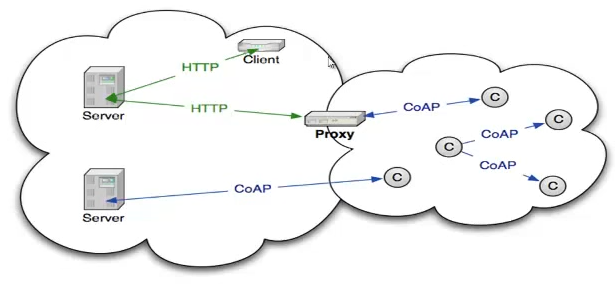
\includegraphics[scale=0.8]{images/coap_architecture.png}
\caption{CoAP Architektur \cite{Shelby14}}
\end{figure}
  
Durch die massgeschneiderten Features für IoT wird CoAP hauptsächlich in WSN's eingesetzt \cite{Obermaier15}. 

\subsection{Publish/Subscribe}
Beim Publish/Subscriber Pattern gibt es einen Sender (Publisher) und einen Empfänger (Subscriber). Der Empfänger hört auf gewisse Themen (Topics). Dies kann nur ein Thema sein oder auch viele Verschiedene. Der Sender kategorisiert seine Nachrichten in Themen und sendet diese zu den jeweiligen Empfänger. Der Sender und der Empfänger wissen aber nichts voneinander. Sie senden oder hören nur im Netzwerk, ob eine für sie interessante Nachricht angekommen ist. Durch die einfache Verknüpfung von Publisher und Subscriber, eignet sich dieses Verfahren sehr gut im IoT-Bereich. Die Sensoren sind die Publisher, sie liefern zum Beispiel Temperaturdaten in die richtige Kategorie. Alle Server/Clouddienste, welche sich für Temperaturdaten interessieren, können auf dieses Kategorie hören. Durch die einfache Handhabung, skaliert dieses Pattern sehr gut.

In der folgenden Grafik sieht man das Publish and Subscribe Pattern. Der Publisher hat eine ''Address Changed'' Message in den Channel geschickt. Nun erhalten alle Subscriber, welche dem Channel folgen, diese Nachricht und verarbeiten sie.

\begin{figure}[H]
\centering
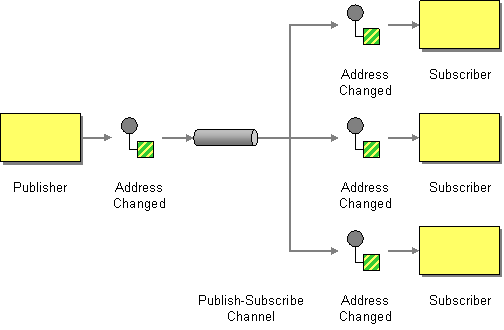
\includegraphics[scale=0.65]{images/publishsubscribe.png}
\caption{Publish and Subscribe Pattern\cite{PublishSubscribePattern}}
\end{figure}
\subsubsection{MQTT}
MQTT (Message Queue Telemetry Transport) ist ein von IBM entwickeltes Protokoll. Es ist ein speziell für IoT entwickeltes Protokoll um Machine-to-Machine Kommunikation herzustellen. Bei dem Protokoll wurde speziell auch ein schlankes Design geachtet. So ist die kleinst Mögliche Nachricht 2 Byte gross. 

Der Hauptverwendungszweck von MQTT ist vorallem der Austausch von Daten zwischen Geräten und Server (D2S).\cite{ProtPubSub} Da das Protokoll für die D2D Konnektivität entwickelt wurde, wird es auch in diesem Bereich eingesetzt. Das heisst die Vorteile liegen in Netzen mit vielen kleinen Geräten, welche wenig Kommunizieren und sich als Kollektion sehen.\cite{ProtPubSubReason}

Bei MQTT wird ein Broker verwendet. Der Sensor ''published'' seine Daten mit einem Topic und den Daten an den Broker. Dieser sendet die Nachricht an alle, welche sich auf das gewünschte Topic Subscribed haben. Durch das schlanke Design, gibt es natürlich auch Nachteile. Aber bei kleinen und einfachen Systemen ist MQTT ein beliebtes Protokoll.
\subsubsection{AMQP}
AMQP (Advanced Message Queuing Protocol) ist ein bekanntes und viel eingesetztes Protokoll. Das binäre Netzwerkprotokoll wird von vielen grossen Firmen\cite{ProtPubSubReason} entwickelt, wie zum Beispiel Microsoft oder auch Cisco. Momentan ist die Version 1.0 seit 2010 als aktuellen Standard im Einsatz.

AMQP wird durch sein Queuing Design im Server zu Server Bereich eingesetzt (S2S).\cite{ProtPubSub} Daher ist es in Bereichen einzusetzen, in der die Geschwindigkeit und der Prozessor nicht relevant sind. Zusätzlich wird es in Bereichen eingesetzt, in dem eine Nachricht nur von A nach B gesendet werden soll und man keine Nachricht verlieren möchte.

Die Sensoren senden die Nachrichten an einen Message Broker, welcher die Nachricht in die richtige Queue schiebt. Nun können sich die Dienste an der Queue anmelden und die Nachrichten konsumieren. Dabei gibt es die Möglichkeit Topics zu setzen, um Kategorien einzuführen. Es können jeder Nachricht auch noch Attribute hinzugefügt werden, wie zum Beispiel Name oder Durability. Durch den grossen Funktionsumfang des Protokolls ist es natürlich auch schwieriger einzurichten und die minimale Paketgrösse wächst damit auch. Die kleinstmögliche Paketgrösse ist 60 Byte.
\subsubsection{XMPP}
XMPP (Extensible Messaging and Presence Protocol) wurde speziell für das Internet der Dinge erweitert, um den Anforderungen gerecht zu werden. XMPP gibt es schon seit mehreren Jahren und wurde in vielen Chatprogrammen eingesetzt. Auch heute findet man das Protokoll beim Facebook-Messenger wieder. Mit der IoT-Erweiterung/Anpassung will man nun nicht mehr Menschen miteinander verknüpfen, sondern Dinge. 

XMPP ist das beste Protokoll um Geräte mit Menschen zu verbinden. Dies ist eine Spezialform des Geräte zu Server Pattern (D2S). \cite{ProtPubSub} XMPP sollte dann verwendet werden, wenn die Geschwindigkeit und der Prozessor nicht wichtig sind, wenn das Gerät immer verbunden sein soll und wenn nur wenige Konnektivitätspunke in einem grossen Bereich vorhanden sind.\cite{ProtPubSubReason}

Bei XMPP wird kein Broker, sondern ein zentraler Server verwendet. Dieser soll allerlei verschiedene Geräte miteinander verbinden. Dieses Protokoll wird häufig für das Remote Management von Konsumergeräten verwendet.
